\documentclass[11pt,a4paper]{article}

\usepackage{amsmath,amssymb,amsthm}
\usepackage{booktabs}
\usepackage{graphicx}
\usepackage{tikz}
\usepackage[margin=1in]{geometry}
\usepackage{fancyhdr}
\usepackage{hyperref}

\pagestyle{fancy}
\fancyhf{}
\renewcommand{\headrulewidth}{0pt}
\fancyfoot[L]{\footnotesize\texttt{two\_theorem\_draft.pdf} --- draft of 22 November 2026, not for circulation}
\fancyfoot[R]{\footnotesize\thepage}

\newtheorem{theorem}{Theorem}
\newtheorem{lemma}[theorem]{Lemma}
\newtheorem{corollary}[theorem]{Corollary}
\theoremstyle{remark}
\newtheorem{remark}[theorem]{Remark}

\newcommand{\C}{\mathbb{C}}
\newcommand{\Z}{\mathbb{Z}}
\newcommand{\Q}{\mathbb{Q}}
\newcommand{\CK}{\mathrm{CK}\text{-}31}
\newcommand{\braket}[2]{\langle#1|#2\rangle}

\title{Coordinate alphabets for Kochen--Specker sets in dimension three:\\
two exact results}
\author{Michael Kernaghan}
\date{Draft, 22 November 2026\\[2pt]{\small file: \texttt{two\_theorem\_draft.pdf}}}

\begin{document}
\maketitle
\thispagestyle{fancy}

\begin{abstract}
The classic three-dimensional Kochen--Specker (KS) proofs draw their ray coordinates from a small
set of numbers: $\{0,\pm1,\pm\sqrt2\}$ for the 33 rays of Peres, $\{0,\pm1,\pm2\}$ for the 31 rays
of Conway and Kochen.  We take that set, the \emph{alphabet}, as the generating object and ask
which alphabets generate an uncolorable pool of rays.  Two families are settled exactly.
(A)~The pool generated by $\{0\}$ and the $n$th roots of unity is KS-uncolorable if and only if
$6\mid n$.  (B)~For every complex $x$ with $|x|^2=2$, the pool generated by
$\{0,\pm1,\pm x,\pm x^{*}\}$ is KS-uncolorable; one fixed list of 45 words is uncolorable at every
point of that circle, collapses to a 33-ray set of Peres type at $x=\sqrt2$ and at $x=\sqrt{-2}$,
and passes through the ring of integers of $\Q(\sqrt{-7})$ on the way.  Away from the circle the
same pool is colorable for generic~$x$: exactly 12 of its 378 orthogonalities depend on
$|x|^2=2$, and they are the ones that matter.
\end{abstract}

\section{The alphabet of a Kochen--Specker set}

The Kochen--Specker theorem~\cite{KochenSpecker1967} is proved by exhibiting a finite set of rays
with no $\{0,1\}$ coloring in which two orthogonal rays are never both~1 and every orthogonal
triad carries exactly one~1 (for a review see~\cite{Budroni2022}).  In dimension three the
smallest known set is the 31-ray configuration of Conway and Kochen ($\CK$), reported by
Peres~\cite{Peres1993}; the best lower bound is~24~\cite{LiBrightGanesh2024,KirchwegerPeitlSzeider2023}.

Peres drew his two three-dimensional examples as cubes~\cite{Peres1991,Peres1993}: each ray joins
the centre of a cube to a marked point on its surface.  The two drawings differ in one respect
only.  In both, the marked points lie on a $5\times5$ grid on each face; for the 33-ray set the
grid lines sit at $0,\pm1,\pm\sqrt2$ and for $\CK$ at $0,\pm1,\pm2$
(Fig.~\ref{fig:triptych}).  This suggests treating the list of coordinate values as a parameter.

\begin{figure}[t]
\centering
\includegraphics[width=\textwidth]{figures/alphabet_cube_triptych.pdf}
\caption{One cube, three alphabets $\{0,\pm1,\pm x\}$ with $x$ real.  Each of the 49 rays of the
pool leaves the centre through a grid point (antipodal points are the same ray).  Filled points:
the 33 rays of Peres ($x=\sqrt2$) and the 31 rays of Conway and Kochen ($x=2$).  At $x=\sqrt3$ the
whole pool is colorable.  Only the two inner grid lines move with~$x$.  The picture is for real
$x>1$; it does not represent the complex pools of Section~\ref{sec:circle}.}
\label{fig:triptych}
\end{figure}

\begin{figure}[t]
\centering
\includegraphics[width=0.62\textwidth]{figures/alphabet_cube_generic.pdf}
\caption{Words as rays.  A ray whose coordinates form a word over $\{0,\pm1,\pm x\}$ leaves the
centre of the cube $[-x,x]^3$ through a grid point of a face; a bar denotes a minus sign.  Words
without the letter $x$, such as $(1,0,0)$ and $(1,\bar1,1)$, reach the surface after scaling
by~$x$.  For example $(x,1,1)\perp(x,\bar1,\bar1)$ exactly when $x^2-1-1=0$.}
\label{fig:generic}
\end{figure}

\paragraph{Definitions.}  An \emph{alphabet} is a finite set $\mathcal A\subset\C$ containing~0.
A \emph{word} is a nonzero element of $\mathcal A^3$, and the \emph{pool} of $\mathcal A$ is the
finite set of rays
\[
S(\mathcal A)=\{\,[v] : v\in\mathcal A^3\setminus\{0\}\,\},
\]
where $[v]$ is the projective class of~$v$ (Fig.~\ref{fig:generic}).  Rays are orthogonal when
$\braket vw=\sum_k v_k^{*}w_k=0$; a \emph{triad} is three mutually orthogonal rays.  A
\emph{coloring} of a set of rays is a map to $\{0,1\}$ such that no two orthogonal rays both
receive~1 and every triad in the set has exactly one~1.  A set with no coloring is
\emph{uncolorable}.

Two cautions fix the scope of everything below.  First, uncolorability is a property of a pool,
not of a ring or a field: every ring considered here contains $\Z$ and hence the coordinates of
$\CK$.  Second, the size of a generator is not an invariant of the pool: multiplying every word by
$x^{-1}$ shows $S(\{0,\pm1,\pm x\})=S(\{0,\pm1,\pm x^{-1}\})$.  Our statements are therefore about
named alphabets and the finite pools they generate.

A coloring of a set restricts to a coloring of any subset, since every orthogonal pair and every
triad of the subset is one of the larger set.  We use this repeatedly:

\begin{lemma}[Restriction]\label{lem:restrict}
A set of rays containing an uncolorable subset is uncolorable.
\end{lemma}

\section{Roots of unity: uncolorable exactly when $6\mid n$}

Let $\zeta_n=e^{2\pi i/n}$, let $\mu_n$ be the group of $n$th roots of unity, and put
$S_n=S(\{0\}\cup\mu_n)$.

\begin{lemma}\label{lem:sums}
A sum of two elements of $\mu_n$ can vanish if and only if $2\mid n$.  A sum of three can vanish
if and only if $3\mid n$, and then the three terms are $\beta,\beta\omega,\beta\omega^2$ with
$\omega$ a primitive cube root of unity.
\end{lemma}

\begin{proof}
$\zeta^a+\zeta^b=0$ iff $\zeta^{b-a}=-1$, and $-1\in\mu_n$ iff $2\mid n$.  For three terms divide
by the first: $1+e^{i\theta}+e^{i\phi}=0$.  The imaginary part gives $\phi=-\theta$ or
$\phi=\pi+\theta$; the second makes the real part~1.  With $\phi=-\theta$ the real part gives
$\cos\theta=-\tfrac12$, so the other two terms are $\omega$ and $\omega^2$, which lie in $\mu_n$
iff $3\mid n$.
\end{proof}

Hence two rays of $S_n$ are orthogonal only if the number of coordinates where both are nonzero
is~0, or~2 with $2\mid n$, or~3 with $3\mid n$.

\begin{theorem}\label{thm:A}
$S_n$ is KS-uncolorable if and only if $6\mid n$.
\end{theorem}

\begin{proof}
\emph{If.}  For $6\mid n$ we have $S_6\subseteq S_n$.  The pool $S_6$ contains the 33-ray set of
Cabello~\cite{Cabello2025simplest}, whose coordinates lie in $\{0,\pm1,\pm\omega,\pm\omega^2\}$
and which is uncolorable.  Apply Lemma~\ref{lem:restrict} twice.

\emph{Only if.}  Let $6\nmid n$.  Write $e_1,e_2,e_3$ for the axis rays.

\emph{Case 1: $2\nmid n$, $3\nmid n$.}  Orthogonal rays have disjoint supports, so the only triad
is $\{e_1,e_2,e_3\}$.  Color $e_1$ with~1 and every other ray with~0.

\emph{Case 2: $2\mid n$, $3\nmid n$.}  Two rays with three common nonzero coordinates are never
orthogonal.  A triad cannot contain an all-nonzero ray~$a$: each of its two partners would share exactly two
nonzero coordinates with~$a$, so would have support of size~2; two such supports meet, so the
partners, being orthogonal to each other, would have the same support; and then $a$ would be
orthogonal to a basis of that coordinate plane and vanish on it.  Rays whose supports are
different two-element sets share one coordinate and are not orthogonal.  So every triad is $\{e_1,e_2,e_3\}$ or $\{e_k,v,v'\}$ with $v,v'$ in the coordinate plane
orthogonal to~$e_k$.  In such a plane the rays are $(1,\zeta^p)$ and $(1,\zeta^p)\perp(1,\zeta^q)$
iff $q-p\equiv n/2$: a perfect matching.  Color $e_1$ with~1 and $e_2,e_3$ with~0; color every
ray of the plane orthogonal to $e_1$ with~0; in each of the other two coordinate planes color one
ray of each matched pair with~1 and the other with~0; color every all-nonzero ray with~0.  Rays in
different coordinate planes share one nonzero coordinate and are not orthogonal, and no ray
colored~1 in those planes is orthogonal to~$e_1$, so no two rays colored~1 are orthogonal, and
each triad has exactly one~1.

\emph{Case 3: $3\mid n$, $2\nmid n$.}  Orthogonality needs common support 0 or~3.  A ray with
exactly one zero coordinate is therefore orthogonal only to the axis ray on its zero coordinate,
and lies in no triad.  For an all-nonzero ray normalise $v=(1,a,b)$.  By Lemma~\ref{lem:sums} an
all-nonzero $w$ is orthogonal to $v$ iff $w=w_{\pm}=(1,a\omega^{\pm1},b\omega^{\mp1})$, and
$\braket{w_+}{w_-}=1+\omega^{-2}+\omega^{2}=0$.  So the all-nonzero rays fall into disjoint triads
with no further orthogonalities among them, and none is orthogonal to a ray with a zero
coordinate.  Color one ray of each such triad with~1, color $e_1$ with~1, and everything else~0.
\end{proof}

The two primes do different work: $3\mid n$ creates triads, $2\mid n$ couples them.  At $n=9$ and
$n=15$ the pool has 28 and 76 triads and is colorable because they are pairwise disjoint
(Table~\ref{tab:cyc}).  The fields $\Q(\zeta_3)$ and $\Q(\zeta_6)$ coincide while $S_3$ is
colorable and $S_6$ is not: Theorem~\ref{thm:A} is a statement about alphabets, not fields.

\begin{table}[t]
\centering
\caption{Cyclotomic pools, exact arithmetic (exponents modulo $n$), colorability by SAT.
Checked for all $2\le n\le20$; a selection is shown.}
\label{tab:cyc}
\begin{tabular}{rrrrc@{\qquad\qquad}rrrrc}
\toprule
$n$ & Rays & Pairs & Triads & Colorable & $n$ & Rays & Pairs & Triads & Colorable\\
\midrule
3 & 21 & 21 & 4 & yes & 12 & 183 & 633 & 67 & \textbf{no}\\
4 & 31 & 69 & 7 & yes & 15 & 273 & 273 & 76 & yes\\
5 & 43 & 18 & 1 & yes & 16 & 307 & 843 & 25 & yes\\
6 & 57 & 174 & 22 & \textbf{no} & 18 & 381 & 1380 & 136 & \textbf{no}\\
9 & 111 & 111 & 28 & yes & 20 & 463 & 1293 & 31 & yes\\
\bottomrule
\end{tabular}
\end{table}

\section{The circle $|x|^2=2$}\label{sec:circle}

The alphabets of Peres and of the $\Z[\sqrt{-2}]$ analogue are $\{0,\pm1,\pm x\}$ with
$x=\sqrt2$ and $x=\sqrt{-2}$.  Both satisfy $|x|^2=2$, and in both the conjugate $x^{*}$ is
already a letter ($x^{*}=\pm x$).  For other $x$ on the circle the natural alphabet is the
conjugate-closed one,
\[
\mathcal A(x)=\{0,\pm1,\pm x,\pm x^{*}\},\qquad P(x)=S(\mathcal A(x)).
\]

\begin{theorem}\label{thm:B}
Let $W$ be the list of 45 words in Table~\ref{tab:words}.
\begin{enumerate}
\item[(i)] For every $x\in\C$ with $|x|^2=2$ the rays of $W$ form a KS-uncolorable set.
Consequently $P(x)$ is uncolorable for every such~$x$.
\item[(ii)] The orthogonalities of $P(x)$ that hold for every $x\in\C$ form a colorable
configuration (145 rays, 366 pairs, 22 triads).  Hence $P(x)$ is colorable for every $x$ outside a finite union of proper real
algebraic subsets of~$\C$.
\end{enumerate}
\end{theorem}

\begin{proof}
The inner product of two words is a polynomial in $x$ and $x^{*}$ with integer coefficients, of
degree at most~2.

(i)  On the circle, $x x^{*}=2$ reduces every such polynomial to an integer combination of
$1,x,x^{*},x^2,x^{*2}$.  With $x=\sqrt2e^{i\theta}$ these are constant multiples of
$e^{ik\theta}$, $k=0,\pm1,\pm2$, which are linearly independent functions of~$\theta$.  So an
inner product vanishes at every point of the circle if and only if every reduced coefficient is
zero, a finite check in integers.  It yields 98 pairs among the words of $W$ that are orthogonal
at every point of the circle, forming the 22 triads listed in the Appendix.  A SAT solver shows
that the configuration with these 98 exclusions and 22 triads has no coloring.  Fix $x$ on the
circle.  If the 45 words give 45 distinct rays, the orthogonality graph at $x$ contains the 98
pairs, and any further pairs or triads only add constraints, so there is no coloring.  If two
words give the same ray, a coloring at $x$ assigns them the same value, and so would also be a
coloring of the 45-vertex configuration; there is none.  (Two words that are orthogonal for every
$x$ on the circle cannot coincide at any of them.)

(ii)  Without the relation, the monomials $x^ax^{*b}$ are linearly independent functions on~$\C$,
so an inner product vanishes for all $x$ iff all coefficients vanish.  This yields 366 pairs and
22 triads on the 145 rays, and a SAT solver finds a coloring.  Each of the remaining inner
products, and each $2\times2$ minor deciding whether two of the 145 words give the same ray, is a
nonzero polynomial in $x,x^{*}$ and vanishes only on a proper real algebraic subset; away from
those finitely many subsets the coloring found is a coloring of $P(x)$.
\end{proof}

\begin{table}[t]
\centering
\caption{The 45 words of Theorem~\ref{thm:B}.  A bar is a minus sign and $x^{*}$ is the complex
conjugate: $\bar x^{*}=-x^{*}$.  The list is one critical set found by greedy reduction (every
single deletion is colorable in the generic graph); it is not known to be the smallest.}
\label{tab:words}
\small
\input{figures/modulus2_words.tex}
\end{table}

\paragraph{What the circle carries.}  On the circle $P(x)$ has 145 rays, 378 pairs and 34
triads at a generic phase.  Comparing with part~(ii), exactly 12 pairs depend on the relation
$|x|^2=2$; each is of the form $1+1-x^{*}x=0$, as in $(x,1,1)\perp(x,\bar1,\bar1)$, and with
them come 12 further triads.  All other orthogonalities are common to every $x$.  The identity that Peres's
cube uses at $x=\sqrt2$ is therefore the whole story along the circle.

\begin{corollary}\label{cor:points}
\begin{enumerate}
\item[(a)] At $x=\sqrt2$ and at $x=\sqrt{-2}$ the 45 words of $W$ give exactly 33 distinct rays,
an uncolorable subset of the 49-ray pool $S(\{0,\pm1,\pm x\})$.  At $x=\sqrt2$ these are the 33
rays of Peres: the other 16 rays of that pool lie in no triad, and a ray in no triad can always be
colored~0, so no uncolorable set of minimum size contains one.
\item[(b)] At $x=(1+\sqrt{-7})/2$ the pool $P(x)$ is the 145-ray pool over the ring of integers of
$\Q(\sqrt{-7})$; it is uncolorable because $|x|^2=2$.
\item[(c)] The words $(1,1,x)$ and $(1,0,x^{*})$ of $W$ have squared overlap
$|1+x^{*2}|^2/12=(5+4\cos2\theta)/12$, which is not constant.  The sets of part~(i) are therefore
not all unitarily equivalent: the circle carries a continuum of inequivalent KS sets.
\end{enumerate}
\end{corollary}

\begin{figure}[t]
\centering
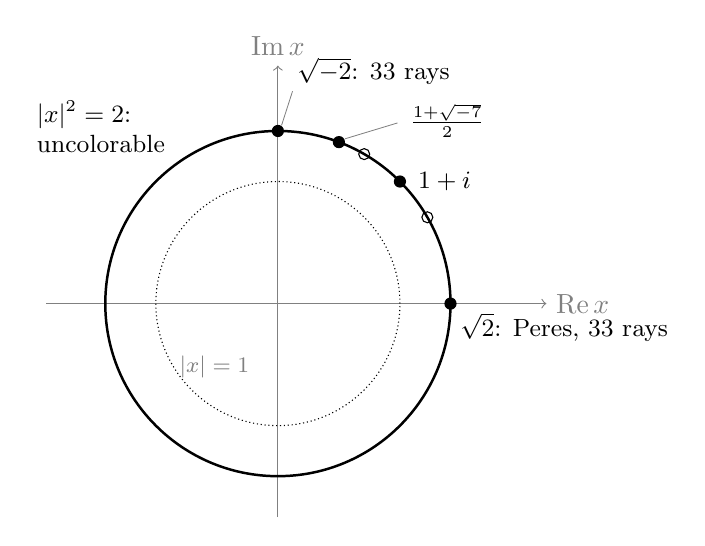
\begin{tikzpicture}[scale=1.55]
\draw[->,gray] (-1.9,0) -- (2.2,0) node[right] {$\mathrm{Re}\,x$};
\draw[->,gray] (0,-1.75) -- (0,1.95) node[above] {$\mathrm{Im}\,x$};
\draw[line width=0.9pt] (0,0) circle (1.4142);
\draw[densely dotted] (0,0) circle (1);
\node[font=\footnotesize,gray] at (-0.52,-0.52) {$|x|=1$};
\fill (1.4142,0) circle (0.05) node[below right,font=\small] {$\sqrt2$: Peres, 33 rays};
\fill (0,1.4142) circle (0.05);
\node[font=\small,anchor=south west] at (0.08,1.72) {$\sqrt{-2}$: 33 rays};
\draw[gray,line width=0.3pt] (0.03,1.46) -- (0.12,1.74);
\fill (1,1) circle (0.05) node[right=3pt,font=\small] {$1+i$};
\fill (0.5,1.3229) circle (0.05);
\node[font=\small,anchor=west] at (1.0,1.5) {$\tfrac{1+\sqrt{-7}}{2}$};
\draw[gray,line width=0.3pt] (0.55,1.35) -- (0.98,1.48);
\draw (1.2247,0.7071) circle (0.045);
\draw (0.7071,1.2247) circle (0.045);
\node[font=\small,align=left] at (-1.45,1.45) {$|x|^2=2$:\\uncolorable};
\end{tikzpicture}
\caption{The alphabet $\{0,\pm1,\pm x,\pm x^{*}\}$ generates an uncolorable pool at every point of
the circle $|x|^2=2$ (the pool is unchanged by $x\mapsto-x$ and $x\mapsto x^{*}$, so one quadrant
suffices).  Filled points: the alphabets of Peres and of $\Z[\sqrt{-2}]$, where the 45 words
collapse to 33 rays, and two points where extra orthogonalities appear.  Open points
($\theta=\pi/6,\pi/3$) also gain orthogonalities in a floating-point survey.}
\label{fig:circle}
\end{figure}

\begin{remark}
Along the circle the graph is not constant.  At $x=(1+\sqrt{-7})/2$ the relation $x+x^{*}=1$
adds orthogonalities, and a floating-point computation gives 522 pairs and 42 triads there against
378 and 34 generically; similar jumps occur at $\theta=\pi/6$, $\pi/4$ and $\pi/3$
(Fig.~\ref{fig:circle}).  The 43-ray set previously extracted from the $\Q(\sqrt{-7})$ pool is
smaller than 45 and presumably uses those extra relations.
\end{remark}

\begin{remark}
The two-symbol alphabet $\{0,\pm1,\pm x\}$ is not the right object for complex~$x$.  Without
$x^{*}$ its pool was colorable at every phase tested other than $0$ and $\pi/2$ (floating-point
survey), including $x=(1+\sqrt{-7})/2$.
\end{remark}

\section{What is and is not claimed}

Proved: Theorem~\ref{thm:A}, by hand.  Proved with computer assistance: Theorem~\ref{thm:B} and
Corollary~\ref{cor:points}, where the orthogonality identities are checked in integer arithmetic
and the two colorability statements are decided by a SAT
solver~\cite{AudemardSimon2018} on instances of 45 and 145 variables
(\texttt{ks\_modulus2\_circle.py} in the repository).  Measured only: Table~\ref{tab:cyc} beyond
what Theorem~\ref{thm:A} implies, and the counts in the two remarks.

Not claimed: that 45 is the least number of rays uncolorable along the whole circle; that the
alphabet construction exhausts the sources of KS sets; that anything here bears on the gap
between 24 and~31.

\paragraph{Draft notes (to be resolved or removed before circulation).}
\begin{enumerate}
\item Gould and Aravind~\cite{GouldAravind2010} exhibit a phase family through Peres's 33 rays.
The family of Theorem~\ref{thm:B} has 45 rays at a generic point and a different graph, but the
relation between the two has not been worked out, and no claim of novelty should be made until it
has.  The same applies to the later analysis of that family by Flores Gordillo.
\item 45 was reached by all 200 greedy descents; a certified minimum is not available.
\item The SAT results should be accompanied by a checkable proof of unsatisfiability and by the
explicit coloring for part~(ii).
\item The counts quoted in the two remarks are floating-point and should be redone exactly.
\item The uncolorability of Cabello's 33-ray set is taken from~\cite{Cabello2025simplest}; an
independent check of the 33 words belongs in the repository.
\end{enumerate}

\paragraph{Acknowledgments.}  Computations, proofs and text were produced with a large language
model (Claude, Anthropic) under the author's direction and reviewed adversarially with a second
model (GPT, OpenAI).  The author is responsible for the content.  Code:
\url{https://github.com/michaelkernaghan/contextuality}.

\begin{thebibliography}{99}
\bibitem{KochenSpecker1967} S.~Kochen and E.~P.~Specker, J.\ Math.\ Mech.\ \textbf{17}, 59 (1967).
\bibitem{Budroni2022} C.~Budroni, A.~Cabello, O.~G\"uhne, M.~Kleinmann, and J.-{\AA}.~Larsson,
Rev.\ Mod.\ Phys.\ \textbf{94}, 045007 (2022).
\bibitem{Peres1991} A.~Peres, J.\ Phys.\ A \textbf{24}, L175 (1991).
\bibitem{Peres1993} A.~Peres, \textit{Quantum Theory: Concepts and Methods} (Kluwer, Dordrecht,
1993), Fig.~7.2 and Plate~II.
\bibitem{LiBrightGanesh2024} Z.~Li, C.~Bright, and V.~Ganesh, in \textit{Proc.\ IJCAI-24},
pp.~1898--1906.
\bibitem{KirchwegerPeitlSzeider2023} M.~Kirchweger, T.~Peitl, and S.~Szeider, in
\textit{Proc.\ IJCAI-23}, pp.~1944--1953.
\bibitem{Cabello2025simplest} A.~Cabello, ``Simplest Kochen--Specker set,'' arXiv:2508.07335.
\bibitem{GouldAravind2010} E.~Gould and P.~K.~Aravind, Found.\ Phys.\ \textbf{40}, 1096 (2010).
\bibitem{AudemardSimon2018} G.~Audemard and L.~Simon, Int.\ J.\ Artif.\ Intell.\ Tools
\textbf{27}, 1840001 (2018).
\end{thebibliography}

\appendix
\section{The 22 triads of the 45 words}
Numbers refer to Table~\ref{tab:words}.  These are the triads that hold at every point of the
circle; the 98 pairs are produced by the script.

\smallskip\noindent\raggedright
\input{figures/modulus2_triads.tex}

\end{document}
